The regular observations of solar flares in Soft and Hard X-ray points towards the "thick-target" interpretation \citep{brown71} of flare accelerated electron injection into the Chromosphere. \cite{brown_2003} coined the source-integrated density weighted mean electron flux $\langle nVF\rangle(E)~[\mathrm{e^{-}cm^{-2}s^{-1}keV^{-1}}]$. The observed hard X-ray spectrum then can be expresses as

%%%%%%%
\begin{equation}\label{e1}
    I(\epsilon)~=~\frac{I}{4\pi R^{2}}\int_{\epsilon}^{\infty}~Q(\epsilon,E)\langle nVF\rangle(E)dE~\propto~\epsilon^{-\gamma}
\end{equation}
%%%%%%%

\noindent where R is the distance between the observed and the Sun, and $Q(\epsilon,E)$ is the angle-averaged bremsstrahlung cross section. The usual cold thick target model gives the relation between the mean electron flux and the injected electron rate as 

%%%%%%
\begin{equation}\label{e2}
    \langle nVF\rangle(E)~=~\frac{E}{K}\int_{E}^{\infty}\dot{N}(E_{0})dE_{0}
\end{equation}
%%%%%%

\noindent $K~=~2\pi e^{4}ln(\Lambda)$ is the collision parameter, e is the electron charge in esu and $ln(\Lambda)$ is the Coulomb logarithm\citep{spitzer62}. The limitations of the standard "thick-target model" becomes more evident when we try to define the accelerated electron spectrum from eqn.~\ref{e1} and \ref{e2} we get

%%%%%%
\begin{equation}
    \dot{N}(E)~=~\dot{N_{0}}\frac{\delta-1}{E_c}\left (\frac{E}{E_c}\right )^{-\delta}
\end{equation}
%%%%%%

\noindent where $\delta~=~\gamma+1$. Here, $E_c$ is an arbitrary reference energy called the low energy cutoff, to stop the total rate of injected electron, $\dot{N_0}~=~\int_{E_c}^{\infty}~\dot{N}(E_{0})dE_0[s^{-1}]$ from diverging. The associated total power in the electron is given as

%%%%%
\begin{equation}
    P[keV.s^{-1}]~=~\int_{E_c}^{\infty}E_0N(E_0)dE_0~=~\frac{1}{\delta-2}E_c^{2-\delta}[\dot{N(E_c)}E_c^{\delta}]~=~\frac{\delta-1}{\delta-2}E_c\dot{N_0}
\end{equation}
%%%%%

\noindent As a consequence various physical properties become very strongly dependent on the low energy cut off. The low energy cut off results in non-physical discontinuous electron distribution of a Maxwellian and power law electron distribution. There are several different attempts to mitigate the nonphysical divergence of the thick target power law injection of electrons at lower energies. \cite{kontar15, kontar19} assumed a warm-target corona and cold chromosphere and included energy diffusion, transport and thermalization of the injected electrons through a warm layer of plasma on top of the cold target to rewrite eq.~\ref{e2} as

%%%%%
\begin{align}
    \langle nVF\rangle(E)~&=~\frac{E}{2K}e^{-E/k_{B}T}\int_{E_{min}}^{E}\frac{e^{E_0/k_{B}T}}{E_0G(\sqrt{E_0/k_{B}T})}~dE_0~\times \int_{E_0}^{\infty} \dot{N}(E_0)~dE_0 \notag \\
    &\simeq~\Delta EM\sqrt{\frac{8}{\pi m_e}}\frac{E}{(k_B T)^{3/2}}e^{-E/k_B T}~+~\frac{E}{K}\int_{E}^{\infty}~\dot{N}(E_0)~dE_0
\end{align}
%%%%%

\noindent where $\Delta EM$ is the "thermalized emission measure" which is created via the thermalization of the electrons and can be written as

%%%%%%
\begin{equation}
    \Delta EM~\simeq~\frac{\pi}{K}\sqrt{\frac{m_e}{8}}(k_B T)^{2}\frac{\dot{N_0}}{E_{min}^{1/2}}~\mathrm{where}~E_{min}~\simeq~3k_B T\left( \frac{5\lambda}{L} \right)^4
\end{equation}
%%%%%%

\noindent where $\lambda~=~(k_B T)^{2}/2Kn$ is the collisional mean free path of the injected electrons. The half loop length L, temperature T and number density n are the physical parameters associated with the coronal loops, through which the electrons are injected. This is known as the "warm target model". Although this model still features a low energy cutoff to the injected electron spectrum, the cutoff is now not ad hoc, and determined by the collisional parameters of the electrons through the coronal loops which in turn are determined by the physical thermal properties of the coronal loops. While the warm target model attempts to explain the physical significance of the low energy cutoff, the use of a $\kappa$-distribution injection of electrons has also proven to be very promising. The $\kappa$-distribution is regularly used to model the electron spectrum in in-situ observations and magnetic reconnection events in the Earth atmosphere \citep{maksimovic05, imada11}.

Close to the low energy cut off usually it is expected that Langmuir waves will be generated and grow\citep{emslie84, hannah09}. The interaction between the waves and the injected electron would flatten the energy energy distribution around the low energy cut off. To reflect this various studies \citep{kasparova09, bataglia15, effenberger17} have used the Kappa distribution, consisting of a Maxwellian core and smoothly merged power-law tail, along with a prominent thermal component to fit the observed X-ray spectrum. Apart from not requiring an arbitrary low-energy cutoff $E_c$, the kappa distribution can provide crucial information on the finer details of the electron acceleration, including the physical conditions of the chromosphere ({\it e.g.} wave-particle interaction, beam-plasma interaction etc.) responsible for the origin of it. \cite{bian14, arnold21} demonstrated that, in presence of Coulomb collisions and velocity diffusion the stochastic acceleration of electrons during solar flares can result in $\kappa$-distribution. In addition, as the $\kappa$-distribution covers the complete energy spectrum and is well behaved throughout, it can provide information about the electrons at a very low energies, which is not sensitive to exchange instruments but can be observed via diagnostics from EUV observations.

\cite{bian14} derived the $\kappa$-distribution as a result of stochastic acceleration in collisional plasma as 

%%%%%%
\begin{equation}\label{e5}
    f_k(v)~=~\frac{n_k}{\pi^{3/2}v_{te}^{3}\kappa^{3/2}}\frac{\Gamma(\kappa)}{\Gamma(\kappa-\frac{3}{2})}\left(1+\frac{v^{2}}{\kappa v_{te}^{2}}\right)^{-\kappa}
\end{equation}
%%%%%%
\noindent where $\kappa~=~\tau_{acc}/2\tau_{c}$ is the kappa index, the ratio of acceleration and collisional decelerations time scale, $v_{te}$ is the thermal speed ($\frac{1}{2}m_ev_{te}^{2}~=~k_{B}T_{\kappa}$). The injected electron rate spectrum and the velocity distribution of the injected electron is given by, $\dot{N}(E)~dE~=~Avf_{k}(v)~d^{3}v$, where A is the injection area. For an isotropic electron distribution ($d^{3}v~=~4\pi v^{2}dv$), plugging in eqn.~\ref{e5} we get:

%%%%%
\begin{equation}\label{e6}
    \dot{N}(E)~=~A\sqrt{\frac{8}{\pi m_{e}k_{B}T_{\kappa}}}\frac{n_k \Gamma(\kappa)}{\Gamma(\kappa-\frac{3}{2})}\frac{E/k_{B}T_{\kappa}}{(1+E/\kappa k_{B}T_{\kappa})^{\kappa}}
\end{equation}
%%%%%

\noindent where $n_{k}[cm^{-3}]~=~\int f_{k}(v)~d^{3}v$ is the total electron number density. So, the total electron injection rate is given by

%%%%%
\begin{equation}\label{e7}
    \dot{N_{0}}~=~\int_{0}^{\infty}\dot{N}(E)~dE~=~2An_k\sqrt{\frac{2k_{B}T_{\kappa}}{m_e}}\frac{\kappa^{1/2}}{(\kappa-2)B(\kappa-3/2,1/2)}
\end{equation}
%%%%%

\noindent pluggin eqn.~\ref{e7} back into eqn.~\ref{e6} we get,

%%%%
\begin{equation}
    \dot{N}(E)~=~\frac{\dot{N_0}}{k_{B}T_{\kappa}}\frac{(\kappa-1)(\kappa-2)}{\kappa^2}\frac{E/k_{B}T_{\kappa}}{(1+E/\kappa k_{B}T_{\kappa})^{\kappa}}
\end{equation}
%%%%

\noindent the associated total power in the electrons is given by, 

%%%%%%
\begin{equation}
    P~=~\int_0^{\infty}E_{0}N(E_{0})~dE_{0}~=~\frac{2\dot{N_{0}}k_BT_{\kappa}\kappa}{\kappa-3}
\end{equation}
%%%%%%

%%%%%%%%%%
\begin{figure}
    \centering
    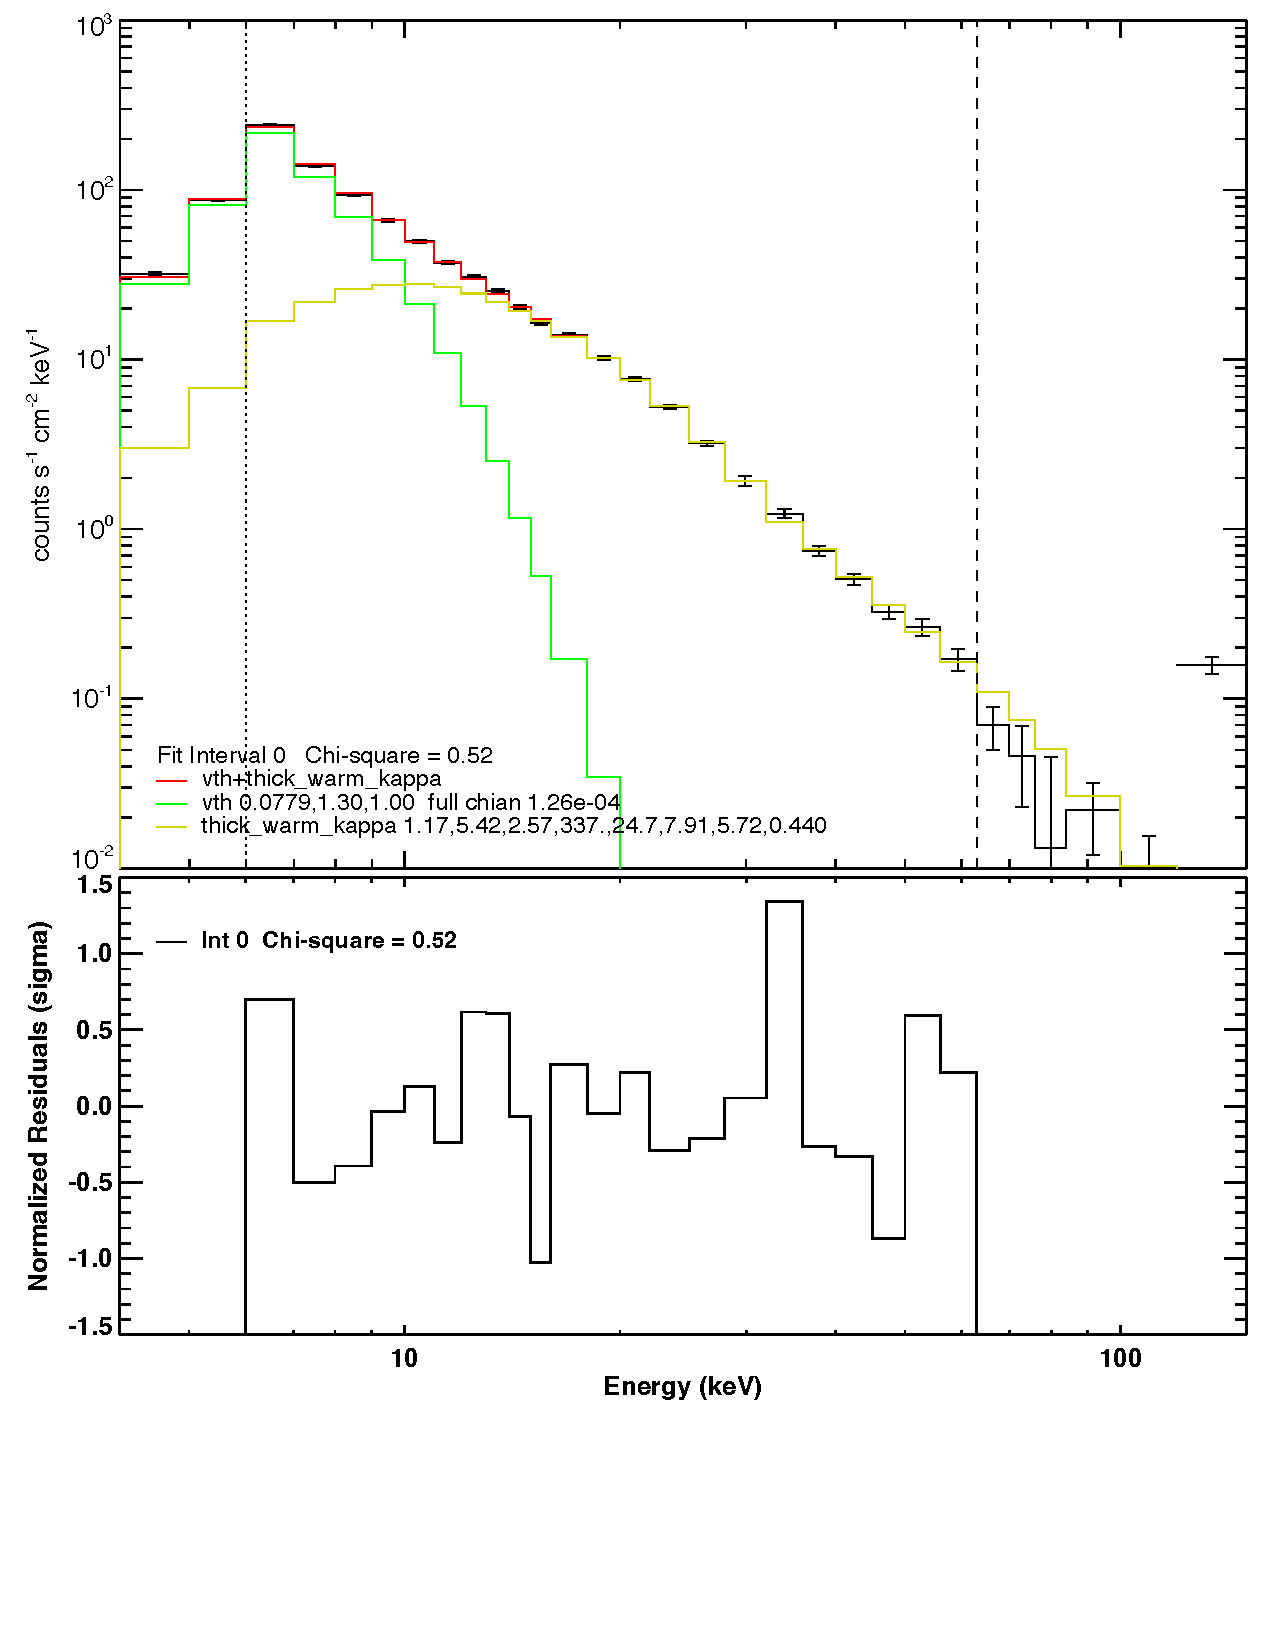
\includegraphics[trim={0.3cm 4cm 0.2cm 0.2cm}, clip, width=0.95\linewidth]{Figures/fit_kappa.pdf}
    \caption{Top panel: STIX spectra integrated between 15:27:00{--}15:27:10~UT during impulsive phase, fitted with `\textit{thcik\_warm\_kappa}' (solid yellow), `\textit{vth}' (solid green) and the complete fit function `\textit{vth+thick\_warm\_kappa}' (solid red line). Bottom panel: The residue of the fit of the STIX spectra.}
    \label{fig:fit_kappa}
\end{figure}
%%%%%%%%%%

We fit the STIX spectra in the same time window as shown in Fig.~\ref{fig:stix_an} with a {\it vth+thick\_warm} and {\it vth+thick\_warm\_kappa} model to compare the two models. We show the {\it vth} (solid green) + {\it warm kappa} electron injection model (solid yellow) fit in Fig.~\ref{fig:fit_kappa} top panel. Fig.~\ref{fig:fit_kappa} lower panel shows the normalized residual of the fit. In Tab.~\ref{tab:my_label} we list the relevant fit parameters from the two respective models. We show the inferred electron injection rate as a function of the electron energy for the {\it warm target+ power law-electron} injection (solid blue) and {\it warm target+ $\kappa$-electron} injection (dashed red) in Fig.~\ref{fig:e-injection} from the fit parameters listed in Tab.~\ref{tab:my_label} for the two distinct electron models. The key thing to notice is the very similar behavior of the models at the higher energy end. The power law injection model goes to 0 very abruptly at the lower energy cutoff ($E_c$), while the kappa distributed electrons slowly taper off at the lower energy end, providing a more physical picture of the injected electron spectra.

%%%%%%%%%%%
\begin{table}[ht!]
    \centering
    \resizebox{0.6\textwidth}{!}{%
    \begin{tabular}{||lcc||}
    \hline
        Parameters & {\it vth+thick\_warm\_kappa} & {\it vth+thick\_warm}\\
    \hline
     & &  \\
       EM[$10^{49}~cm^{-3}$] & 0.078 & 0.078\\
        &  &   \\
       $k_{B}T[keV]$ & 1.30 & 1.30\\
        & &  \\
       $\dot{N_0}[10^{35}~e^{-1}.s^{-1}]$ & 1.17 & 1.89\\
        & &  \\
        $\delta$ & NA & 3.21 \\
         & &  \\
        $\kappa$ & 5.42 & NA \\
         & &  \\
         $E_c$ & NA & .76\\
          & &  \\
        $k_{B}T_{\kappa}$ & 2.57 & NA \\
         & & \\
         
    \hline
    \end{tabular}}
    \caption{Comparison of various model parameters between "{\it vth+thick2}", "{\it vth+thick\_warm}" and "{\it vth+thick\_warm\_kappa}" model for the same time window of STIX spectra as shown in Fig.~\ref{fig:stix_an}.}
    \label{tab:my_label}
\end{table}
%%%%%%%%%%%

%%%%%%
\begin{figure}
    \centering
    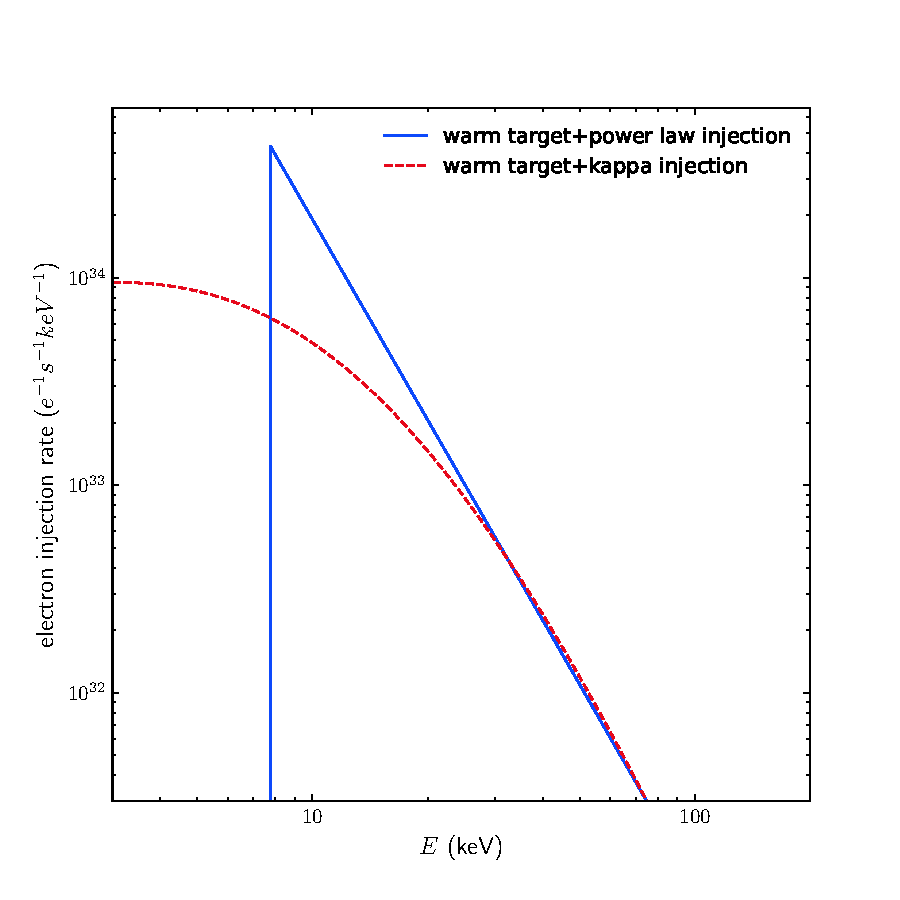
\includegraphics[width=0.8\linewidth, trim={0cm 0cm 1cm 1cm}, clip]{Figures/e_ij.pdf}
    \caption{Inferred electron injection rate as a function of energy for power law electron injection (solid blue) and $\kappa$-distributed electron injection (dashed red) from the fit parameters listed in Tab.~\ref{tab:my_label}.}
    \label{fig:e-injection}
\end{figure}
%%%%%%